\subsection{¿Que es el protocolo HTTP?}
The Hypertext Transfer Protocol (HTTP) is a stateless application-level 
request/response protocol that uses extensible semantics and
   self-descriptive message payloads for flexible interaction with
   network-based hypertext information systems.
   HTTP is a generic interface protocol for information systems.  It is
   designed to hide the details of how a service is implemented by
   presenting a uniform interface to clients that is independent of the
   types of resources provided.  Likewise, servers do not need to be
   aware of each client's purpose: an HTTP request can be considered in
   isolation rather than being associated with a specific type of client
   or a predetermined sequence of application steps.  The result is a
   protocol that can be used effectively in many different contexts and
   for which implementations can evolve independently over time.
  
   One consequence of this flexibility is that the protocol cannot be
   defined in terms of what occurs behind the interface.  Instead, we
   are limited to defining the syntax of communication, the intent of
   received communication, and the expected behavior of recipients.  If
   the communication is considered in isolation, then successful actions
   ought to be reflected in corresponding changes to the observable
   interface provided by servers.  However, since multiple clients might
   act in parallel and perhaps at cross-purposes, we cannot require that
   such changes be observable beyond the scope of a single response.
   
\subsection{Arquitectura}
HTTP was created for the World Wide Web (WWW) architecture and has
evolved over time to support the scalability needs of a worldwide
hypertext system.  Much of that architecture is reflected in the
terminology and syntax productions used to define HTTP.

\subsubsection*{Client/Server Messaging}

HTTP is a stateless request/response protocol that operates by
exchanging messages across a reliable transport- or
session-layer "connection".  An HTTP "client" is a
program that establishes a connection to a server for the purpose of
sending one or more HTTP requests.  An HTTP "server" is a program
that accepts connections in order to service HTTP requests by sending
HTTP responses.
Most HTTP communication consists of a retrieval request (GET) for a
representation of some resource identified by a URI.  In the simplest
case, this might be accomplished via a single bidirectional
connection (===) between the user agent (UA) and the origin
server (O).



\begin{center}
   \begin{figure}   
      \begin{center}
         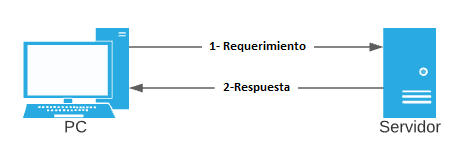
\includegraphics{2.1.png}
      \end{center}
      \caption{Simple comunication method}
   \end{figure}
\end{center}


A client sends an HTTP request to a server in the form of a request
message, beginning with a request-line that includes a method, URI,
and protocol version, followed by header fields
containing request modifiers, client information, and representation
metadata, an empty line to indicate the end of the
header section, and finally a message body containing the payload
body (if any, Section 3.3).
A server responds to a client's request by sending one or more HTTP
   response messages, each beginning with a status line that includes
   the protocol version, a success or error code, and textual reason
   phrase (Section 3.1.2), possibly followed by header fields containing
   server information, resource metadata, and representation metadata
   (Section 3.2), an empty line to indicate the end of the header
   section, and finally a message body containing the payload body (if
   any, Section 3.3).
\subsubsection*{Ejemplo}
The following example illustrates a typical message exchange for a
GET request (Section 4.3.1 of [RFC7231]) on the URI
"http://www.example.com/hello.txt":

Client request:

  GET /hello.txt HTTP/1.1
  User-Agent: curl/7.16.3 libcurl/7.16.3 OpenSSL/0.9.7l zlib/1.2.3
  Host: www.example.com
  Accept-Language: en, mi


Server response:

  HTTP/1.1 200 OK
  Date: Mon, 27 Jul 2009 12:28:53 GMT
  Server: Apache
  Last-Modified: Wed, 22 Jul 2009 19:15:56 GMT
  ETag: "34aa387-d-1568eb00"
  Accept-Ranges: bytes
  Content-Length: 51
  Vary: Accept-Encoding
  Content-Type: text/plain

  Hello World! My payload includes a trailing CRLF.

  HTTP is defined as a stateless protocol, meaning that each request
   message can be understood in isolation.  Many implementations depend
   on HTTP's stateless design in order to reuse proxied connections or
   dynamically load balance requests across multiple servers.  Hence, a
   server MUST NOT assume that two requests on the same connection are
   from the same user agent unless the connection is secured and
   specific to that agent.  Some non-standard HTTP extensions (e.g.,
   [RFC4559]) have been known to violate this requirement, resulting in
   security and interoperability problems.

    
 


\subsection{Métodos mas importantes del del protocolo HTTP}

head 
delete      
CONNECT
OPTIONS
TRACE
PUT

4.3.1.  GET

   The GET method requests transfer of a current selected representation
   for the target resource.  GET is the primary mechanism of information
   retrieval and the focus of almost all performance optimizations.
   Hence, when people speak of retrieving some identifiable information
   via HTTP, they are generally referring to making a GET request.

   It is tempting to think of resource identifiers as remote file system
   pathnames and of representations as being a copy of the contents of
   such files.  In fact, that is how many resources are implemented 
   .  However, there are
   no such limitations in practice.  The HTTP interface for a resource
   is just as likely to be implemented as a tree of content objects, a
   programmatic view on various database records, or a gateway to other
   information systems.  Even when the URI mapping mechanism is tied to
   a file system, an origin server might be configured to execute the
   files with the request as input and send the output as the
   representation rather than transfer the files directly.  Regardless,
   only the origin server needs to know how each of its resource
   identifiers corresponds to an implementation and how each
   implementation manages to select and send a current representation of
   the target resource in a response to GET.


4.3.3.  POST

   The POST method requests that the target resource process the
   representation enclosed in the request according to the resource's
   own specific semantics.  For example, POST is used for the following
   functions (among others):

   o  Providing a block of data, such as the fields entered into an HTML
      form, to a data-handling process;
      o  Posting a message to a bulletin board, newsgroup, mailing list,
      blog, or similar group of articles;

   o  Creating a new resource that has yet to be identified by the
      origin server; and

   o  Appending data to a resource's existing representation(s).


\subsection{Response Status Codes} 
The status-code element is a three-digit integer code giving the
   result of the attempt to understand and satisfy the request.

   HTTP status codes are extensible.  HTTP clients are not required to
   understand the meaning of all registered status codes, though such
   understanding is obviously desirable.  However, a client MUST
   understand the class of any status code, as indicated by the first
   digit, and treat an unrecognized status code as being equivalent to
   the x00 status code of that class, with the exception that a
   recipient MUST NOT cache a response with an unrecognized status code.

   For example, if an unrecognized status code of 471 is received by a
   client, the client can assume that there was something wrong with its
   request and treat the response as if it had received a 400 (Bad
   Request) status code.  The response message will usually contain a
   representation that explains the status.

   The first digit of the status-code defines the class of response.
   The last two digits do not have any categorization role.  There are
   five values for the first digit:

   o  1xx (Informational): The request was received, continuing process

   o  2xx (Successful): The request was successfully received,
      understood, and accepted

   o  3xx (Redirection): Further action needs to be taken in order to
      complete the request

   o  4xx (Client Error): The request contains bad syntax or cannot be
      fulfilled
      o  5xx (Server Error): The server failed to fulfill an apparently
      valid request
  

\subsection{HTTPS con SSL} 

With an understanding of some of the key concepts of cryptography,
we can now look closely at the operation of the Secure Sockets Layer
(ssl) protocol. Although ssl is not an extremely complicated protocol, 
it does offer several options and variations. 
The ssl protocol consists of a set of messages and rules about when
to send (and not to send) each one. In this chapter, we consider what
those messages are, the general information they contain, and how
systems use the different messages in a communications session. 

\subsubsection*{SSL Roles}
The Secure Sockets Layer protocol defines two different roles for the
communicating parties. One system is always a client, while the other
is a server. The distinction is very important, because ssl requires the
two systems to behave very differently. The client is the system that
initiates the secure communications; the server responds to the client’s request. 
In the most common use of ssl, secure Web browsing,
the Web browser is the ssl client and the Web site is the ssl server.
For ssl itself, the most important distinctions between clients and
servers are their actions during the negotiation of security parameters. 
Since the client initiates a communication, it has the
responsibility of proposing a set of ssl options to use for the
exchange. The server selects from the client’s proposed options,
deciding what the two systems will actually use. Although the final
decision rests with the server, the server can only choose from among
those options that the client originally proposed.

\subsubsection*{SSL Messages}
When ssl clients and servers communicate, they do so by exchanging ssl messages. 
this chapter will show how systems use these messages in their communications.
The most basic function that an ssl client and server can perform is
establishing a channel for encrypted communications. 
This section looks at these steps
in more detail by considering each message in the exchange.


GRAFIQUITO DE LOS MENSAJES 

\paragraph*{ClientHello}
The ClientHello message starts the ssl communication between the
two parties. The client uses this message to ask the server to begin
negotiating security services by using ssl. 

The Version field of the ClientHello message contains the highest
version number of ssl that the client can support. The current ssl
version is 3.0, and it is by far the most widely deployed on the Internet. 

The RandomNumber field, as you might expect, contains a random
number. This random value, along with a similar random value that
the server creates, provides the seed for critical cryptographic calculations.
  The ssl specification suggests that
four of this field’s 32 bytes consist of the time and date. 

The next field in the ClientHello message is SessionID. Although all
ClientHello messages may include this field, in this example, the
field is meaningless and would be empty. 
The CipherSuites field allows a client to list the various cryptographic
services that the client can support, including exact algorithms and
key sizes. The server actually makes the final decision as to which
cryptographic services will be used for the communication, but it is
limited to choosing from this list. 

The CompressionMethods field is, in theory, similar to the CipherSuites field.
 In it, the client may list all of the various data compression methods that 
 it can support. Compression methods are an
important part of ssl because encryption has significant consequences on the 
effectiveness of any data compression techniques. Encryption changes the 
mathematical properties of information in a
way that makes data compression virtually impossible. 

\paragraph*{ServerHello}
When the server receives the ClientHello message, it responds with a
ServerHello. 
The Version field is the first example of a server making a final 
decision for the communications. The ClientHello’s version simply identifies 
which ssl versions the client can support. The ServerHello’s
version, on the other hand, determines the ssl version that the communication
 will use. 
The RandomNumber field of the ServerHello is essentially the same
as in the ClientHello, though this random value is chosen by the
server. Along with the client’s value, this number seeds important
cryptographic calculations. 
The SessionID field of a ServerHello may contain a value, unlike the
ClientHello’s field just discussed. The value in this case uniquely
identifies this particular ssl communication, or session. The main reason for 
explicitly identifying a particular ssl session is to refer to it
again later.
The CipherSuite field (note that the name is singular, not plural, as in
the case of a ClientHello) determines the exact cryptographic parameters, 
specifically algorithms and key sizes, to be used for the session. 
The server must select a single cipher suite from among those
listed by the client in its ClientHello message.
The CompressionMethod field is also singular for a ServerHello. In
theory, the server uses this field to identify the data compression to
be used for the session. Again, the server must pick from among
those listed in the ClientHello. Current ssl versions have not defined
any compression methods, however, so this field has no practical utility.

\paragraph*{ServerKeyExchange}
In this example, the server follows its ServerHello message with a
ServerKeyExchange message. This message complements the CipherSuite field 
of the ServerHello. While the CipherSuite field indicates
the cryptographic algorithms and key sizes, this message contains the
public key information itself. The exact format of the key information depends
 on the particular public key algorithm used. For the rsa
algorithm, for example, the server includes the modulus and public
exponent of the server’s rsa public key.
Note that the ServerKeyExchange message is transmitted without
encryption, so that only public key information can be safely included within it.
 The client will use the server’s public key to encrypt
a session key, which the parties will use to actually encrypt the application
 data for the session.
\paragraph*{ServerHelloDone}
The ServerHelloDone message tells the client that the server has finished with
 its initial negotiation messages. The message itself contains no other 
 information, but it is important to the client, because
once the client receives a ServerHelloDone, it can move to the next
phase of establishing the secure communications.
\paragraph*{ClientKeyExchange}
When the server has finished its part of the initial ssl negotiation,
the client responds with a ClientKeyExchange message. Just as the
ServerKeyExchange provides the key information for the server, the
ClientKeyExchange tells the server the client’s key information. In

this case, however, the key information is for the symmetric encryption 
algorithm both parties will use for the session. Furthermore, the
information in the client’s message is encrypted using the public key
of the server. This encryption protects the key information as it traverses
 the network, and it allows the client to verify that the server
truly possesses the private key corresponding to its public key. Otherwise,
 the server won’t be able to decrypt this message. This operation is an 
 important protection against an attacker that intercepts
messages from a legitimate server and pretends to be that server by
forwarding the messages to an unsuspecting client. Since a fake
server won’t know the real server’s private key, it won’t be able to decrypt 
the ClientKeyExchange message. Without the information in
that message, communication between the two parties cannot succeed.
\paragraph*{ChangeCipherSpec}
After the client sends key information in a ClientKeyExchange message, 
the preliminary ssl negotiation is complete. At that point, the
parties are ready to begin using the security services they have negotiated.
 The ssl protocol defines a special message—
ChangeCipherSpec—to explicitly indicate that the security services
should now be invoked.
Since the transition to secured communication is critical, and both
parties have to get it exactly right, the ssl specification is very precise
in describing the process. First, it identifies the set of information
that defines security services. That information includes a specific
symmetric encryption algorithm, a specific message integrity algorithm, 
and specific key material for those algorithms. The ssl specification also 
recognizes that some of that information (in particular,
the key material) will be different for each direction of communication. 
In other words, one set of keys will secure data the client sends
to the server, and a different set of keys will secure data the server
sends to the client. (In principle, the actual algorithms could differ as
well, but ssl does not define a way to negotiate such an option.) For
any given system, whether it is a client or a server, ssl defines a write
state and a read state. The write state defines the security information

for data that the system sends, and the read state defines the security
information for data that the system receives.
The ChangeCipherSpec message serves as the cue for a system to
begin using its security information. Before a client or server sends a
ChangeCipherSpec message, it must know the complete security information it 
is about to activate. As soon as the system sends this
message, it activates its write state. Similarly, as soon as a system receives
 a ChangeCipherSpec from its peer, the system activates its
read state.

GRAFIQUITO Figures 3-2 and 3-3

\paragraph*{Finished}
Immediately after sending their ChangeCipherSpec messages, each
system also sends a Finished message. The Finished messages allow
both systems to verify that the negotiation has been successful and
that security has not been compromised. Two aspects of the Finished
message contribute to this security. First, as the previous subsection
explained, the Finished message itself is subject to the negotiated cipher suite. 
That means that it is encrypted and authenticated according to that suite.
 If the receiving party cannot successfully decrypt
and verify the message, then clearly something has gone awry with
the security negotiation.
The contents of the Finished message also serve to protect the security of the
 ssl negotiation. Each Finished message contains a cryptographic hash of 
 important information about the just-finished
negotiation.  Notice that protected data includes the exact content of all
handshake messages used in the exchange (though ChangeCipherSpec messages 
are not considered “handshake” messages in the strict
sense of the word, and thus are not included). This protects against
an attacker who manages to insert fictitious messages or remove 
legitimate messages from the communication. If an attacker were able
to do so, the client’s and server’s hash calculations would not match,
and they would detect the compromise.

\paragraph*{Ending Secure Communications}

Although as a practical matter it is rarely used (primarily due to the
nature of Web sessions), ssl does have a defined procedure for ending a
 secure communication between two parties. In this procedure,
 the two systems each send a special ClosureAlert to the other.
Explicitly closing a session protects against a truncation attack, in
which an attacker is able to compromise security by prematurely terminating
 a communication. 

\subsubsection*{Authenticating the Server’s Identity}
previously it was explained how ssl can establish encrypted
communications between two parties, that may not really add that
much security to the communication. With encryption alone neither
party can really be sure of the other’s identity. The typical reason for
using encryption in the first place is to keep information secret from
some third party. But if that third party were able to successfully
masquerade as the intended recipient of the information, then encryption 
would serve no purpose. The data would be encrypted, but
the attacker would have all the data necessary to decrypt it.
To avoid this type of attack, ssl includes mechanisms that allow each
party to authenticate the identity of the other. With these mechanisms, 
each party can be sure that the other is genuine, and not a
masquerading attacker. In this section, we’ll look at how ssl enables a
server to authenticate itself.
A natural question is, of course, if authenticating identities is so important,
 why don’t we always authenticate both parties? 
 Aca un ejemplo que sirva en una red interna
 The answer
lies in the nature of Web commerce. When you want to purchase
something using your Web browser, it’s very important that the Web
site you’re browsing is authentic. You wouldn’t want to send your
credit card number to some imposter posing as your favorite merchant. 
The merchant, on the other hand, has other means for
authenticating your identity. Once it receives a credit card number,
for example, it can validate that number. Since the server doesn’t
need ssl to authenticate your identity, the ssl protocol allows for
server authentication only. 

\paragraph*{Certificate}
When authenticating your identity, the server sends a Certificate message 
in place of the ServerKeyExchange message previously described. The Certificate 
message simply contains a certificate chain
that begins with the server’s public key certificate and ends with the
certificate authority’s root certificate.
The client has the responsibility to make sure it can trust the certificate it 
receives from the server. That responsibility includes verifying
the certificate signatures, validity times, and revocation status. It also
means ensuring that the certificate authority is one that the client
trusts. Typically, clients make this determination by knowing the
public key of trusted certificate authorities in advance, through some
trusted means. Netscape and Microsoft, for example, preload their
browser software with public keys for well-known certificate authorities. 
Web servers that want to rely on this trust mechanism can only
obtain their certificates (at least indirectly) from one of these wellknown
 authorities.

\paragraph*{ClientKeyExchange}
The client’s ClientKeyExchange message also differs in server authentication, 
though the difference is not major. When encryption
only is to be used, the client encrypts the information in the ClientKeyExchange
 using the public key the server provides in its
ServerKeyExchange message. In this case, of course, the server is authenticating
 itself and, thus, has sent a Certificate message instead of
a ServerKeyExchange. The client, therefore, encrypts its ClientKeyExchange information 
using the public key contained in the
server’s certificate. This step is important because it allows the client
to make sure that the party with whom it is communicating actually
possesses the server’s private key. Only a system with the actual private key will 
be able to decrypt this message and successfully continue the communication.

\subsubsection*{Certificate Functionality}

\paragraph*{Single Domain}
As the name suggests, a single domain SSL certificate can only be used on a single 
domain or IP. This is considered the default SSL certificate type. The DV SSL type is
available at all validation levels.
\paragraph*{Multi-Domain}
This SSL type is a jack-of-all-trades certificate. Multi-Domain Wildcards can encrypt
 up to 250 different domains and unlimited sub-domains. Unfortunately, it's not available
  in EV.
\paragraph*{Wildcard}
Wildcards are specifically designed to encrypt one domain and all of its accompanying 
sub-domains. Unlimited sub-domains. Unfortunately, Wildcards are only available at the 
DV and OV levels.
\paragraph*{Multi-Domain Wildcard}
These are the jack-of-all-trades certificates. Multi-Domain Wildcards can encrypt up 
to 250 different domains and unlimited sub-domains. Unfortunately, it's not available 
in EV.

\subsubsection*{Validation Level}
There are three types of SSL Certificate available today; Extended Validation 
(EV SSL), Organization Validated (OV SSL) and Domain Validated (DV SSL). The 
encryption levels are the same for each certificate, what differs is the vetting
 and verification processes needed to obtain the certificate.
\paragraph*{Domain Validation (DV)}
Domain Validation SSL or DV SSL represents the base-level for SSL types. These 
are perfect for websites that just need encryption and nothing more. DV SSL 
certificates are typically inexpensive and they can be issued within minutes. That's 
because the validation process is fully automated. Just prove you own your domain 
and the DV SSL certificate is yours.
\paragraph*{Organization Validation (OV)}
Organization Validation SSL or OV SSL represents the middle ground for SSL certificate 
types. To obtains OV SSL, your company or organization must undergo light business
 vetting. This can take up to three business days because someone has to verify 
 your business information. OV SSL displays the same visual indicators as DV SSL,
  but provides a way for your customers to check your verified business information 
  in the certificate details section.
\paragraph*{Extended Validation (EV)}
Extended Validation SSL or EV SSL requires extensive business vetting by Comodo. This
 may sound like a lot, but it's really not if your business has publicly available 
 records. EV SSL activates a unique visual indicator – your verified organization name
  shown in the browser.

  
\subsubsection*{Identifier Validation Challenges}

(CAMBIAR LA INTRO, NO ME GUSTA LO DE IDENTIFICADOR, RELACIONARLO MAS CON UN DOMINIO)

ACME uses an extensible challenge/response framework for identifier
validation.  The server presents a set of challenges in the
authorization object it sends to a client (as objects in the
"challenges" array), and the client responds by sending a response
object in a POST request to a challenge URL.

   Different challenges allow the server to obtain proof of different
   aspects of control over an identifier.  In some challenges, like HTTP
   and DNS, the client directly proves its ability to do certain things
   related to the identifier.  The choice of which challenges to offer
   to a client under which circumstances is a matter of server policy.


   

\paragraph*{HTTP Challenge}

   With HTTP validation, the client in an ACME transaction proves its
   control over a domain name by proving that it can provision HTTP
   resources on a server accessible under that domain name.  The ACME
   server challenges the client to provision a file at a specific path,
   with a specific string as its content.

   This is the most common challenge type today. The server gives a
   token to your ACME client, and your ACME client puts a file on your web 
   server at {http://\<YOUR\_DOMAIN\>/.well-known/acme-challenge/\<TOKEN\>}. That 
   file contains the token, plus a thumbprint of your account key. 

   Once the client tells to the server that the file is ready, the server 
   tries retrieving it.On receiving a response, the server constructs and stores the key
   authorization from the challenge "token" value and the current client
   account key.

   Given a challenge/response pair, the server verifies the client's
   control of the domain by verifying that the resource was provisioned
   as expected.

   (TAL VEZ PARA LA PRESENTACION)

   Pros:

    It’s easy to automate without extra knowledge about a domain’s configuration.
    It allows hosting providers to issue certificates for domains CNAMEd to them.
    It works with off-the-shelf web servers.

   Cons:

    It doesn’t work if your ISP blocks port 80 (this is rare, but some residential ISPs do this).
    Let’s Encrypt doesn’t let you use this challenge to issue wildcard certificates.
    If you have multiple web servers, you have to make sure the file is available on all of them.

   (EXPLICAR POR QUE NO PUEDO USAR ESTE DESAFIO)

\paragraph*{DNS Challenge}
   When the identifier being validated is a domain name, the client can
   prove control of that domain by provisioning a TXT resource record
   containing a designated value for a specific validation domain name.

   A client fulfills this challenge by constructing a key authorization
   from the "token" value provided in the challenge and the client's
   account key.  The client then computes the SHA-256 digest 
   of the key authorization.

   The record provisioned to the DNS contains the base64url encoding of
   this digest.  The client constructs the validation domain name by
   prepending the label {\_acme-challenge} to the domain name being
   validated, then provisions a TXT record with the digest value under
   that name.  For example, if the domain name being validated is
   "www.example.org", then the client would provision the following DNS
   record:
   \_acme-challenge.www.example.org. 300 IN TXT "gfj9Xq...Rg85nM"
   
   On receiving a response, the server constructs and stores the key
   authorization from the challenge "token" value and the current client
   account key.

   To validate a DNS challenge, the server performs the following steps:

   1.  Compute the SHA-256 digest of the stored key
       authorization

   2.  Query for TXT records for the validation domain name

   3.  Verify that the contents of one of the TXT records match the
       digest value

   If all of the above verifications succeed, then the validation is
   successful.  If no DNS record is found, or DNS record and response
   payload do not pass these checks, then the validation fails.

   The client SHOULD de-provision the resource record(s) provisioned for
   this challenge once the challenge is complete, i.e., once the
   "status" field of the challenge has the value "valid" or "invalid".
